\Chapter{ARTICLE 1 : RESISTANCE WELDING OF THERMOPLASTIC COMPOSITES WITH A NANOCOMPOSITE HEATING ELEMENT}\label{sec:Theme1}

\hyphenation{COMSOL na-no-com-po-si-te na-no-com-po-si-tes}

\selectlanguage{french}
\section{Introduction}

Cet article présente les travaux ayant mené au développement d'un élément chauffant nanocomposite pour le soudage résistif de composites thermoplastiques. La planification des travaux, la réalisation des expériences, l'analyse des résultats et la rédaction de cet article ont été réalisés par David Brassard. Martine Dubé et Jason R. Tavares ont supervisés l'ensemble des travaux et ont contribués à la révision de l'article. 

\textbf{Auteurs} : David Brassard, Martine Dubé et Jason R. Tavares

\textbf{Article publié dans la revue} : Composites Part B: Engineering, Volume 165, 15 May 2019, Pages 779-784

\textbf{URL} : \url{https://doi.org/10.1016/j.compositesb.2019.02.038}

\textbf{Mots clés} : Resistance welding; Polymer–matrix composites (PMCs); Thermoplastic resin; Joints/joining

\selectlanguage{english}

\section{Abstract}

In this study, we propose a new heating element (HE) for the resistance welding of thermoplastic composites. 
This HE is made of polyetherimide (PEI), rendered electrically conductive by the addition of 10\% wt. multi-wall carbon nanotubes (MWCNT) (conductivity of \SI{0.79}{\siemens\per\cm}).
The new HE were successfully used to weld carbon fibre/poly(ether ether ketone) (CF/PEEK) laminates in a single lap shear configuration, leading to a lap shear strength of up to \SI{19.6}{\mega\pascal}.
Observations of the fracture surfaces revealed a cohesive failure mode within the nanocomposite HE and non-uniform heating over the weld area. 
It is believed that PEI/MWCNT HE present an interesting alternative to current HE, although more work is needed to improve the temperature homogeneity over the weld area.
	
%%%%%%%%%%%%%%%%%%%%%%%%%%%%%%%%%%%%%%%%%%%%%%%%%%%%%%%%%%%%%%%%%
\section{Introduction}
%%%%%%%%%%%%%%%%%%%%%%%%%%%%%%%%%%%%%%%%%%%%%%%%%%%%%%%%%%%%%%%%%

The current fierce competition in the space industry is putting a strong downward pressure on the launch cost of satellites. 
New processes and materials are needed to reduce launchers' weight and cost. 
Fibre reinforced polymers are commonly used to achieve weight reduction. 
Currently, thermoset polymers dominate the market for composite matrices but thermoplastic composites (TPC) are attracting the attention of the industry \cite{CompositeWorldSloan2018} because of their higher impact resistance, increased production rates, superior recyclability and higher environmental resistance \cite{cogswell1992}. 
Moreover, a distinct advantage of thermoplastics over thermosets is their ability to be joined by welding instead of adhesive bonding or mechanical fastening. 

Different welding processes have been developed for various applications and joint geometry. 
Resistance welding, induction welding and ultrasonic welding are a few of the processes used for joining TPC. 
To weld the adherents (i.e. the parts to be joined) through traditional resistance welding (Fig. \ref{fig:welding_jig}a), heat is generated by a porous and electrically conductive heating element located at the weld interface and connected to a power source. 
An electrical current is applied to the heating element to generate heat. 
The connection between the power supply and the heating element is generally established by copper connectors that are clamped at a predetermined distance from the edges of the adherents (the so-called “clamping distance”). 
During the welding process, pressure is applied to the weld stack to achieve intimate contact and to promote autohesion during the melting and consolidation phases. 

\begin{figure}[h]
	\centering
	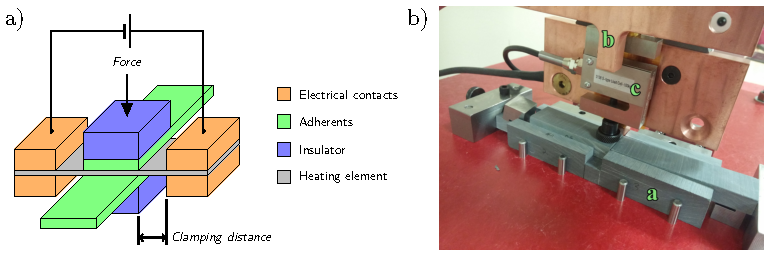
\includegraphics[width=130mm]{Fig1.pdf}
	\caption{Resistance welding jig a) Resistance welding main components, b) Ceramic insulators [a], copper electrodes [b] and load cell [c] \cite{Brassard2018_figshare_article1}}
	\label{fig:welding_jig}
\end{figure}

\FloatBarrier
The first heating elements that were used for the resistance welding process were made of carbon fibre  \cite{Ageorges2000a,houghton1984bonding,Eveno1988}.
Poor weld reproducibility and problematic electrical connections between the electrodes and the carbon fibres caused scaling issues \cite{McKnight1997}. 
These shortcomings led to the use of stainless steel (SS) mesh heating elements that improved the consistency of the process \cite{Hou1999a}.

The lap shear strength (LSS) obtained from single lap shear (SLS) specimens and failure modes are commonly reported to evaluate the performance of welded joints. 
For samples welded with SS heating elements under suboptimal conditions, adhesive failure (ADH) between the mesh and the polymer or between the polymer and the adherents is obtained. 
These failure modes can be accompanied by tearing of the mesh. 
Under good welding conditions, light-fiber-tear failure (LFT), often accompanied by mesh tearing, is observed \cite{Shi2014}. 
Failure modes and LSS are dependent on the fibre nature and orientation within the adherents \cite{Shi2013a}. 
For materials with lower performances, such as glass fibre and polyetherimide (GF/PEI), failure occurs in the adherents, but for high performance and stiffer materials, such as unidirectional carbon fibre and poly(ether ether ketone) (CF/PEEK) laminates, damage occurs in the heating element with little to no damage to the adherents \cite{Dube2015}. 
The variations in the failure modes indicate that poor adhesive bonding between the polymer and the SS mesh can be a limiting factor under certain circumstances \cite{Dube2007,Dube2012a,Dube2009a,Shi2014,Shi2015a}. 
An increase in the fraction of open area of the SS mesh, to a certain extent, improves LSS. 
Concurrently, some concerns were expressed regarding the weight penalty of SS meshes \cite{Stavrov2005a}. 

Players from the space industry are looking at alternative heating elements.  
Their target is a low-density material that is not affected by corrosion. 
A conductive polymer-based nanocomposite heating element, compatible with the adherents, could serve as that alternative and provide good interfacial bonding. 
Such nanocomposites are formed by dispersing conductive nanoparticles (typically metal or carbon) into a polymer matrix. 
The electrical properties of nanocomposites depend, among other things, on the intrinsic properties of the nanoparticles, their mass fraction, surface modifications, and the mixing method employed. 
This was illustrated by Bauhofer et al., who showed that the same kinds of particles can produce nanocomposites with widely different properties \cite{Bauhofer2009}. 
For applications such as resistance welding, we seek a conductivity sufficiently low to generate heat through the Joule effect but high enough to prevent current leakage through the adherents. 

For traditional resistance welding of high performance TPC parts made of CF/PEEK, PEI is sometimes used to provide a resin-rich region at the weld interface. 
The miscibility of PEI in PEEK \cite{Crevecoeur1991} also improves the bonding between the adherents to attain good mechanical performances. 
By using PEI for the matrix of the nanocomposite, we hypothesize that we could take advantage of that miscibility and obtain a nanocomposite heating element suitable for resistance welding of CF/PEEK laminates while welding at temperatures lower than the melting temperature of PEEK (in a similar way to the Thermabond process \cite{Smiley1991a}). 
This novel heating element would be almost entirely miscible within the matrix of the composite and does not leave metallic elements within the weld. 
Furthermore, the MWCNT/PEI coefficient of thermal expansion is better matched with that of CF/PEEK composites than pure PEI with a metallic insert. 
Therefore, it is believed that thermal residual stress can be reduced by the use of this nanocomposite HE. 

This article presents the development of this new heating element for resistance welding of TPC with a PEI-based conductive nanocomposite. 
Joule heating of the nanocomposite is validated with a sample heating element. 
This new heating element is then used to join CF/PEEK adherents and their mechanical performance is evaluated by single lap shear tests. 

%%%%%%%%%%%%%%%%%%%%%%%%%%%%%%%%%%%%%%%%%%%%%%%%%%%%%%%%%%%%%%%%%
\section{Methodology}
%%%%%%%%%%%%%%%%%%%%%%%%%%%%%%%%%%%%%%%%%%%%%%%%%%%%%%%%%%%%%%%%%

%%%%%%%%%%%%%%%%%%%%%%%%%%%%%%%%%%%%%%%%%%%%%%%%%%%%%%%%%%%%%%
\subsection{Materials}
%%%%%%%%%%%%%%%%%%%%%%%%%%%%%%%%%%%%%%%%%%%%%%%%%%%%%%%%%%%%%%

\subsubsection{Polymer and Nanocomposite}

The polymer used for the heating element development was PEI (CAS 61128-46-9) pellets ordered from Sigma Aldrich. 
PEI pellets had a melt index of \SI{18}{\gram} per \SI{10}{\minute} at \SI{337}{\celsius} with a mass of \SI{6.6}{\kilogram}. 
GPC/SEC measurements of the molecular weight for this PEI gave a $M_n$ of \SI{15.0}{\kg\per\mol} and a $M_w$ of \SI{21.6}{\kg\per\mol}. 

The conductive nanoparticles consisted of dry powdered MWCNTs, produced by combustion chemical vapour deposition (CCVD), purchased from Raymor Industries. 
They had outer diameters in the range of \SIrange{10}{20}{\nano\metre}, lengths from \SIrange{1}{12}{\micro\metre} and purity of at least 99\%.

Initial batches of nanocomposites with 5\%, 10\% and 15\% wt. of MWCNTs were produced with a DSM Xplore 5~cc twin-screw micro-compounder. 
Polymer pellets were introduced along with the MWCNTs and internally mixed by the recirculation circuit.
The resulting extruded wire was cut into pellets that were mixed and fed a second time to produce a uniform mix for each batch. 
The pellets were hot-pressed to produce \SI{1.6}{\mm} thick flat samples to measure their electrical conductivity.  

The electrical conductivity of the PEI nanocomposites, at 5\%, 10\% and 15\% wt. of MWCNTs, was measured with the four-point probe technique. 
A probe manufactured by Jandel engineering was mounted on a resistivity test rig from A\&M Fell Ltd. and connected to an acquisition system composed of a Keithley 220 programmable current source and a Hewlett Packard 34401A multimeter. 
The tungsten carbide probes had a diameter of \SI{0.4}{\mm}, a radius of \SI{100}{\um} and a spacing of \SI{1}{\mm}. 

The final batch of nanocomposite with 10\% wt. of MWCNTs, for the manufacturing of the heating elements, was produced in a twin-screw extruder and processed at \SI{340}{\celsius}. 
Polymer pellets were introduced along with the MWCNTs. 
The extruded wire was cut into small pellets, mixed thoroughly and fed back into the extruder two other times to obtain a uniform composition. 
The final wire was cut into pellets prior to further processing. 
Flat PEI nanocomposite heating elements, with a 10\% mass fraction of MWCNTs, were produced by hot pressing pellets into \SI{0.5}{\milli\metre} thick films and cutting them into rectangles of \SI{12.7 x 55}{\milli\metre}. 

\subsubsection{Composite}

The TPC adherents were produced by compression moulding CF/PEEK pre-impregnated plies to form unidirectional (UD) composite laminates and cutting them to dimensions (\SI{25.4 x 101.6}{\milli\metre} ), with an abrasive saw, according to ASTM D5868 - 01(2014). 
In agreement with the supplier’s recommendations, the stacks of plies were heated to \SI{390}{\celsius} under a pressure of \SI{0.25}{\MPa}. 
The pressure was then increased to \SI{1}{\MPa} for \SI{30}{\minute} to consolidate the laminate before cooling it back to room temperature in about \SI{60}{\minute}. 
The pressure was maintained during the cooling phase. 

%%%%%%%%%%%%%%%%%%%%%%%%%%%%%%%%%%%%%%%%%%%%%%%%%%%%%%%%%%%%%%
\subsection{Joule Heating of a Nanocomposite Heating Element}
%%%%%%%%%%%%%%%%%%%%%%%%%%%%%%%%%%%%%%%%%%%%%%%%%%%%%%%%%%%%%%

Prior to the welding tests, a simple validation of the heating elements was devised. 
A \SI{0.5}{\milli\metre} thick PEI heating element was installed in the welding setup and connected to electrodes \SI{25}{\mm} spaced apart. 
A constant DC voltage was then applied for \SI{45}{\s}. 
A FLIR T420 infrared camera was used to record the surface temperature distribution once an electrical current was applied. 

%%%%%%%%%%%%%%%%%%%%%%%%%%%%%%%%%%%%%%%%%%%%%%%%%%%%%%%%%%%%%%
\subsection{Welding Experiments}
%%%%%%%%%%%%%%%%%%%%%%%%%%%%%%%%%%%%%%%%%%%%%%%%%%%%%%%%%%%%%%

A computer-controlled resistance welding jig was built to weld single lap shear specimens with an overlap of \SI{12.7}{\milli\metre} and a width of \SI{25.4}{\milli\metre} (Fig. \ref{fig:welding_jig}). 
Two copper electrodes were used to connect the power source to the nanocomposite heating element. 
Three pneumatic actuators applied constant pressure over the two electrodes and the welding zone, while the nanocomposite was kept between two composite adherents. 
The electrodes where connected to the heating element, on each side of the laminate (Fig. \ref{fig:welding_jig}a) with the proper clamping distance for each test. 
Electrical power was supplied by a \SI{10}{\kW} programmable DC power source series XR from Magna-Power capable of providing up to \SI{160}{\volt} and \SI{60}{\ampere}. 
The power source can be driven as a constant voltage source, constant current source or with custom power profiles. 
A modulation scheme was configured to allow the source to operate with a constant power output. 
In this mode of operation, the source adjusts its output current based on the voltage applied and keeps a constant power output, disregarding variations in the resistance of the heating element. 

For the welding experiments, electrical parameters were set so as to closely mimic conditions that are observed during traditional resistance welding of TPC. 
The initial voltage setting for constant voltage operation was calculated based on a specific power of \SI{350}{\kW\per\square\metre} and the electrical resistance of the heating element. 

Prior to welding, the surfaces of the adherents and the nanocomposite were cleaned with acetone. 
Once the heating element and adherents were installed in the welding jig, a contact pressure of 2.4 MPa was applied by the electrodes on the heating element, to minimize contact resistance. 
Over the weld area, a third actuator applied a constant pressure of \SI{1}{\MPa} during the whole welding process. 
It was previously demonstrated, for traditional resistance welding, that pressures close to \SI{1}{\MPa} are able to produce welds with good mechanical properties by promoting intimate contact, necessary for polymer chain diffusion at the interfaces, while preventing void formation due to excessive polymer flow out of the weld \cite{Ageorges2000a, Dube2007, Shi2014}. 
Type K thermocouples, located on the ceramic above the welded zone, monitored the temperature during the welding process (Fig. \ref{fig:thermocouple}a). 
The thermocouples could not be installed directly on the nanocomposite heating element, as their presence altered the heat transfer mechanisms within the weld and Kapton\textregistered \ tape was not sufficient prevent electrical interference. 
The first thermocouple was located slightly off centre at \SI{14}{\milli\metre} from the edge of the adherent at the centreline of the overlap. 
The second thermocouple was also located on the centreline, but \SI{2.5}{\milli\metre} away from the edge of the adherent. 
These two locations served as proxy to approximate the temperature within the weld. 
Closer to the heating element, a higher temperature is expected. 
Aside from the operating mode for the power source, the clamping distance and the duration of the welding process were the main factors taken into account during the welding tests. 

\begin{figure}[b!]
	\centering
	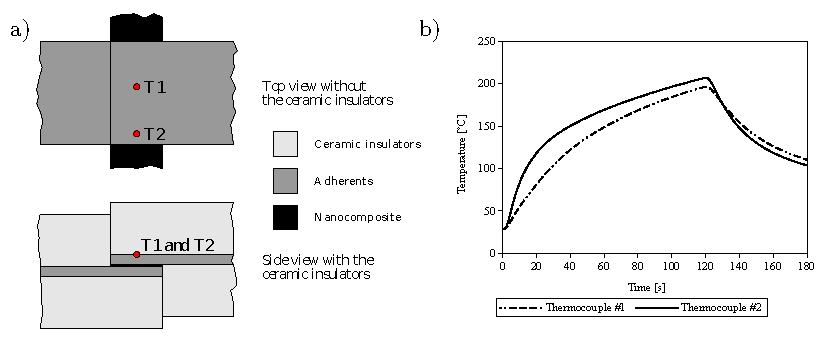
\includegraphics[width=140mm]{Fig2.pdf}
	\caption{Thermocouples locations and measurements a) Location of the thermocouples during the welding process, b) Evolution of the temperature during the welding process at \SI{350}{\kilo\watt\per\square\metre} for \SI{120}{\second} \cite{Brassard2018_figshare_article1}}
	\label{fig:thermocouple}
\end{figure}

\FloatBarrier
%%%%%%%%%%%%%%%%%%%%%%%%%%%%%%%%%%%%%%%%%%%%%%%%%%%%%%%%%%%%%%
\subsection{Characterization of welded joints}
%%%%%%%%%%%%%%%%%%%%%%%%%%%%%%%%%%%%%%%%%%%%%%%%%%%%%%%%%%%%%%

The LSS of each weld was evaluated with a SLS test as per ASTM D5868 – 01(2014) with an MTS Alliance RF/200 testing machine. 
Subsequently, fractography analysis was carried out with ImageJ. 
In this analysis, dividing the area of the welded zone by the total area gave the percentage of welded area. 
Both faces of the fractured specimens were evaluated to get an average measure for each sample. 
The failure modes obtained were classified and reported as per ASTM D5573 – 99(2012). 

%%%%%%%%%%%%%%%%%%%%%%%%%%%%%%%%%%%%%%%%%%%%%%%%%%%%%%%%%%%%%%
\subsection{FTIR Analysis}
%%%%%%%%%%%%%%%%%%%%%%%%%%%%%%%%%%%%%%%%%%%%%%%%%%%%%%%%%%%%%%

FTIR spectra were collected to validate the absence of thermal degradation due to the welding process. 
A Nicolet iS5 FTIR Spectrometer equipped with an iD5 attenuated total reflectance (ATR) module was used to collect spectra from the virgin PEI pellets and PEI nanocomposite films before welding, and PEI nanocomposite on the fracture surfaces after SLS tests. 
Spectra for CF/PEEK adherents were also collected to serve as reference.  

%%%%%%%%%%%%%%%%%%%%%%%%%%%%%%%%%%%%%%%%%%%%%%%%%%%%%%%%%%%%%%%%%
\section{Results and Discussion}
%%%%%%%%%%%%%%%%%%%%%%%%%%%%%%%%%%%%%%%%%%%%%%%%%%%%%%%%%%%%%%%%% 

%%%%%%%%%%%%%%%%%%%%%%%%%%%%%%%%%%%%%%%%%%%%%%%%%%%%%%%%%%%%%%
\subsection{Electrical Conductivity of the Nanocomposites}
%%%%%%%%%%%%%%%%%%%%%%%%%%%%%%%%%%%%%%%%%%%%%%%%%%%%%%%%%%%%%%

The electrical conductivity of PEI nanocomposites with 5\%, 10\% and 15\% wt. MWCNTs was \SIlist[multi-part-units = single]{0.27(08);0.79(06);0.92(30)}{\siemens\per\cm}, respectively. 
It was decided that the marginal gain in conductivity between 10\% and 15\% wt. MWCNTs was not worth the increased cost and production problems associated with high particle loading (such as increased viscosity and brittleness). 
Thus, a PEI nanocomposite with 10\% wt. MWCNTs was retained for manufacturing heating elements. 

%%%%%%%%%%%%%%%%%%%%%%%%%%%%%%%%%%%%%%%%%%%%%%%%%%%%%%%%%%%%%%
\subsection{Micro-Mechanical Simulations of Joule Heating}
%%%%%%%%%%%%%%%%%%%%%%%%%%%%%%%%%%%%%%%%%%%%%%%%%%%%%%%%%%%%%%

During the initial development of the nanocomposite, finite element models were developed using COMSOL Mul\-ti\-phy\-sics\-\textregistered \ to evaluate the contribution of the three main heating mechanisms inside the nanocomposite heating element (i.e. Joule heating of MWCNTs, from the concentration of charges at the contact points between MWCNTs and of the matrix between MWCNTs) and verify that the polymer will not undergo thermal degradation.  
A set of three continuum micromechanic models presenting different contact topologies were used to assess the relative contribution of each heating mechanism to the global heating phenomena within a conductive nanocomposite. 
The uniform temperature fields observed at the constituent level led to the conclusion that under normal operating conditions, local thermal degradation should not occur within the nanocomposite during the welding process and that Joule heating is the dominant mode of heat generation. 
The complete methodology and results for these simulations are included as Supplementary Information. 

%%%%%%%%%%%%%%%%%%%%%%%%%%%%%%%%%%%%%%%%%%%%%%%%%%%%%%%%%%%%%%
\subsection{Joule Heating of a Nanocomposite Heating Element}
%%%%%%%%%%%%%%%%%%%%%%%%%%%%%%%%%%%%%%%%%%%%%%%%%%%%%%%%%%%%%%

At the beginning of the Joule Heating tests, a uniform temperature field is observed in the nanocomposite (Fig. \ref{fig:results_lab}). 
For longer test durations, the copper electrodes are acting as heat sinks at the edges of the heating element causing a measurable temperature gradient (Fig. \ref{fig:results_lab}). 
It was possible to control the surface temperature of the heating element with a variation of the voltage (Tab. \ref{tab:results_lab}). 
The voltages applied during this test were limited to stay below the glass transition temperature of PEI at \SI{217}{\celsius}. 
These results validate the Joule heating behaviour of the nanocomposite heating element. 

\begin{figure}[htb]
	\centering
	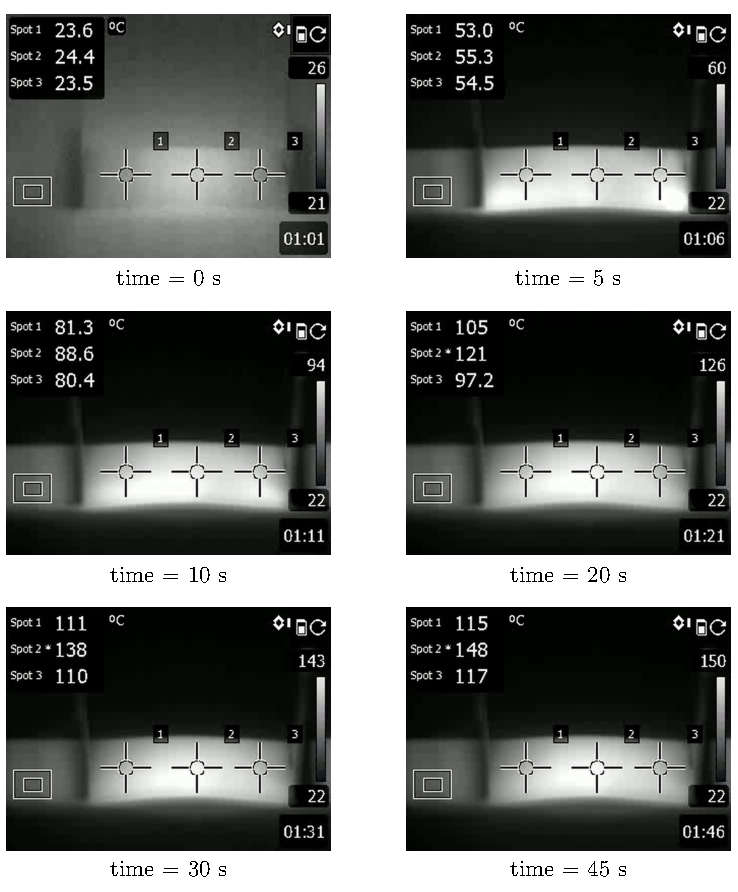
\includegraphics[width=125mm]{Fig3.pdf}
	\caption{Thermography of a heating element during the experimental validation under a DC electrical field of \SI{800}{\volt\per\metre} \cite{Brassard2018_figshare_article1}}
	\label{fig:results_lab}
\end{figure}

\begin{table}[htb]
	\centering
	\caption{Electrical results from the experimental validation, the current at \SI{30}{\volt} could not be measured due to melting of the heating element}
	\begin{tabular}{@{}lrrr@{}}
		\toprule
		Voltage 				& Electric							& Maximum  				& Current\\ 
		& field								& surface 				& \\ 
		& 										& temperature 			& \\
		{[}\si{\volt}{]} 	& {[}\si{\volt\per\metre}{]} 	& {[}\si{\celsius}{]}	& {[}\si{\ampere}{]}\\ \midrule
		10 						& 400									& 44 						& 0.10 \\
		15						& 600									& 97 						& 0.16 \\
		20 						& 800									& 155 						& 0.23 \\
		25 						& 1000									& 223 						& 0.32 \\
		30 						& 1200									& \textgreater 270 	& N/A \\ \bottomrule
	\end{tabular}
	
	\label{tab:results_lab}
\end{table}

\FloatBarrier
%%%%%%%%%%%%%%%%%%%%%%%%%%%%%%%%%%%%%%%%%%%%%%%%%%%%%%%%%%%%%%
\subsection{Welding Experiments}
%%%%%%%%%%%%%%%%%%%%%%%%%%%%%%%%%%%%%%%%%%%%%%%%%%%%%%%%%%%%%%

Small geometric variations of the nanocomposite heating elements (thickness and width) introduced variations of the electrical resistance. 
Because of this variation, operation under constant voltage conditions achieved poor reproducibility between initial welding tests and was not investigated further. 
Operation under constant power yielded significant improvements in the consistency of welding results, avoiding the effect introduced by the heating element electrical resistance variation. 

\subsubsection{Constant power welding}

Tests were carried out at a specific power of \SI{350}{\kW\per\square\metre} with a constant pressure of \SI{1}{\MPa} on the weld. 
Clamping distances of \SIlist{0;1;1.5}{\mm} and welding times of \SIlist{60;70;90;120}{\s} were investigated. 
Three samples were produced for each welding condition. 
The LSS along with the average fraction of welded areas are reported in Table \ref{tab:SLS_and_fractography_results}. 

\begin{table}[h]
	\centering
	\caption{LSS and fractography analysis reported as average values $\pm$ standard deviation \cite{Brassard2018_figshare_article1}}
	\begin{tabular}{@{}lllcccc@{}}
		\toprule
		Clamping distance & Values      &                 &                     \multicolumn{4}{c}{Time}                      \\
		{[}\si{\mm}{]}    &             &                 &                 \multicolumn{4}{c}{{[}\si{\s}{]}}                 \\
		                  &             &                 &       60       &       70       &       90       &      120       \\ \midrule
		0                 & LSS         & {[}\si{\MPa}{]} &                &                &                & \num{14.5(13)} \\
		                  & Welded area & {[}\%{]}        &                &                &                &  \num{85(2)}   \\
		1                 & LSS         & {[}\si{\MPa}{]} &                &                &                & \num{13.0(44)} \\
		                  & Welded area & {[}\%{]}        &                &                &                &  \num{83(7)}   \\
		1.5               & LSS         & {[}\si{\MPa}{]} & \num{16.4(78)} & \num{18.6(20)} & \num{15.5(38)} & \num{19.6(35)} \\
		                  & Welded area & {[}\%{]}        &  \num{57(20)}  &  \num{74(10)}  &  \num{87(1)}   &  \num{78(2)}   \\ \bottomrule
	\end{tabular}
	\label{tab:SLS_and_fractography_results}
\end{table}

\FloatBarrier
Average LSS from \SI{13}{\MPa} up to \SI{19.6}{\MPa} were obtained. 
Longer weld times allowed the nanocomposite to melt and bind with the adherents over a larger fraction of the welded zone. 
From the conditions tested, applying current for \SI{120}{\s} with a clamping distance of \SI{1.5}{\mm} yielded the best LSS results. 

Cohesive failure within the nanocomposite was the primary mode of failure observed for samples welded under constant power with UD composite adherents.
Some adhesive failure on the edges of the heating element was also observed. 
Samples welded for \SI{60}{\s} with a clamping distance of \SI{1.5}{\mm} presented a higher fraction of adhesive failure. 
The zone where cohesive failure is observed had thinner width at the centre of the weld (Fig. \ref{fig:fracture_surface}a). 
For welding times of \SI{90}{\s} and longer, the thinner middle section is absent from the results and only cohesive failure of the nanocomposite is present (Fig. \ref{fig:fracture_surface}b). 

\begin{figure}[h]
	\centering
	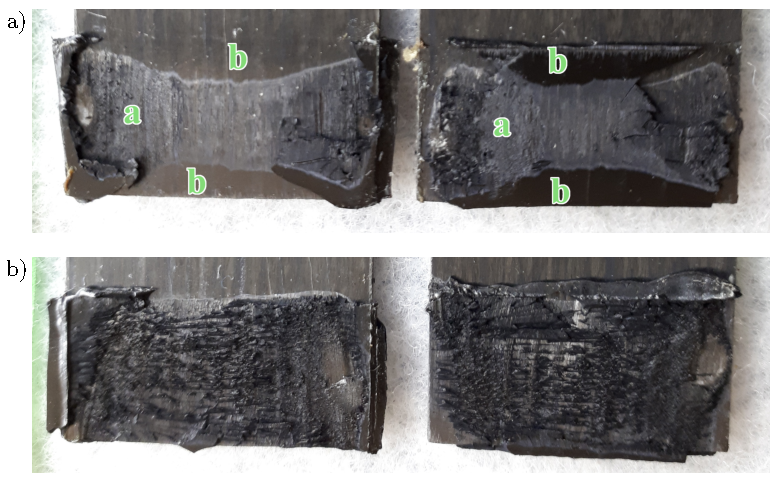
\includegraphics[width=132mm]{Fig4.pdf}
	\caption{Fracture surface of specimens welded at \SI{350}{\kW\per\square\metre} with \SI{1.5}{\mm} clamping distance a) Cohesive failure with a thinner section in the middle [a] and adhesive failure on the sides [b] in a sample welded for \SI{70}{\s}, b) Mostly cohesive failure in a sample welded for \SI{90}{\s} \cite{Brassard2018_figshare_article1}}
	\label{fig:fracture_surface}
\end{figure}

\FloatBarrier
Temperature monitoring during the welding process of a sample with a clamping distance of \SI{1.5}{\mm} showed temperature variations between the centre and the edge of the weld (Fig. \ref{fig:thermocouple}b).
For this specimen, the edge effect resulted in a \SI{10}{\celsius} higher temperature on the top surface at the edge of the adherent, compared to the center. 
This difference was caused by a clamping distance that was too large. 
Models will be required to evaluate if the gradients in the weld are larger or smaller than the gradient from the thermocouples located at the top of the adherents. 
Nonetheless, the temperature gradient between the center and the edges was not large enough to lead to observable thermal degradation in the fractography results, either on the edges (from a too large clamping distances) or at the centre of the weld (from a too small clamping distances). 
It was previously demonstrated that the clamping distance has an important effect on the heat transfer at the edge of the weld \cite{Talbot2013}. 

Although the LSS obtained with the nanocomposite heating element are lower than the best results reported in the literature for traditional resistance welding, successful welds were obtained and key optimization parameters were identified for future work. 
A better understanding and control of those parameters will allow the production of higher performance joints. 
The key parameters are : \begin{enumerate}
	\item the reduced toughness of the nanocomposite due to the addition of a high fraction of MWCNTs,
	\item the incomplete polymer melting in the welded zone due to edge effects and
	\item the thinner middle section in the welded zone leading to stress concentration at the edge. 
\end{enumerate}
Tensile tests on dogbones made from the nanocomposite showed that the addition of 10\% wt. fraction of MWCNTs caused a 40\% reduction of the tensile strength compared to virgin PEI. 
Plasticizers could be used to reduce the negative impact of MWCNTs but the composition of the nanocomposite will need to be balanced so as to still provide a sufficient electrical conductivity. 
Improving the control of the welding process (clamping distance, time and power density) will reduce the temperature gradients within the welded zone and provide a better wetting over the whole surface of the joint. 

\subsection{FTIR results}

When comparing the FTIR spectra of PEI nanocomposites before and after the welding process, no signs of degradation could be noted (see Supplementary Information). 
The characteristic peeks for \ch{CH3}, \ch{CH} and \ch{C=O} in PEI were left unchanged by the welding process. 

%%%%%%%%%%%%%%%%%%%%%%%%%%%%%%%%%%%%%%%%%%%%%%%%%%%%%%%%%%%%%%%%%
\section{Conclusion}
%%%%%%%%%%%%%%%%%%%%%%%%%%%%%%%%%%%%%%%%%%%%%%%%%%%%%%%%%%%%%%%%%

Through this work, we have demonstrated that a PEI/MWCNT-based nanocomposite heating element could be used for resistance welding of TPCs. 
An experimental validation using a PEI/MWCNT flat heating element subjected to a DC electric field showed uniform heating. 
Resistance welding using the PEI/MWCNT heating element in a custom-built welding jig joined CF/PEEK UD panels with LSS up to \SI{19.6}{\MPa}. 
Good bonding to the adherents is supported by the cohesive failure mode observed, and no important thermal degradation is measured by FTIR tests. 
Future work will focus on improving the temperature uniformity in the weld and improving the toughness of the nanocomposite heating element.

%%%%%%%%%%%%%%%%%%%%%%%%%%%%%%%%%%%%%%%%%%%%%%%%%%%%%%%%%%%%%%%%%
\section{Acknowledgements}
%%%%%%%%%%%%%%%%%%%%%%%%%%%%%%%%%%%%%%%%%%%%%%%%%%%%%%%%%%%%%%%%%

This work was supported by ArianeGroup and CREPEC. 
The authors also thank Prof. G.S. Patience for the use of the thermal imaging camera and Prof. D. Therriault for access to the microcompounder. 

%%%%%%%%%%%%%%%%%%%%%%%%%%%%%%%%%%%%%%%%%%%%%%%%%%%%%%%%%%%%%%%%%
\section{Supplementary Information}
%%%%%%%%%%%%%%%%%%%%%%%%%%%%%%%%%%%%%%%%%%%%%%%%%%%%%%%%%%%%%%%%%

%%%%%%%%%%%%%%%%%%%%%%%%%%%%%%%%%%%%%%%%%%%%%%%%%%%%%%%%%%%%%%
\subsection{Continuum Micromechanic Simulations}
%%%%%%%%%%%%%%%%%%%%%%%%%%%%%%%%%%%%%%%%%%%%%%%%%%%%%%%%%%%%%%

In the early phase of the nanocomposite heating elements development, finite element models were developed using COMSOL Mul\-ti\-phy\-sics\-\textregistered \ to verify that the polymer would not undergo thermal degradation and to evaluate the contribution of the three main heating mechanisms inside the nanocomposite heating element (i.e. Joule heating of MWCNTs, from the concentration of charges at the contact points between MWCNTs and of the matrix between MWCNTs).  
A set of three continuum micromechanic models presenting different contact topologies were used to assess the relative contribution of each heating mechanism to the global heating phenomena within a conductive nanocomposite. 
Representative elementary volumes (REV) in which the MWCNTs represented 1\% of the total mass were used in these models (Fig. \ref{fig:geometry}). 

\begin{figure}[htb]
	\centering
	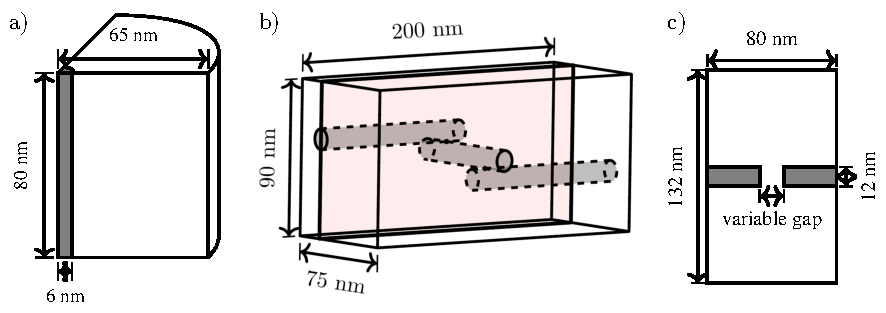
\includegraphics[width=150mm]{Fig1s.pdf}
	\caption{Geometries of the representative elementary volume composed of MWCNT (dark region) and the insulating matrix (white region) a) Quarter view of the revolved 2D axisymmetric FEM simulating the Joule heating within a MWCNT, b) Geometry of the second FEM evaluating the effect of charge concentration at contact point, c) Geometry of the third FEM simulating Joule heating within the polymer matrix \cite{Brassard2018_figshare_article1}}
	\label{fig:geometry}
\end{figure}

\FloatBarrier

In the first model, a single MWCNT (Fig. \ref{fig:geometry}a dark zone), surrounded by PEI (Fig. \ref{fig:geometry}a white zone) was represented using axisymmetric boundary conditions. 
The top and bottom surfaces of the MWCNT acted as voltage source and ground, respectively, with the current flowing through the MWCNT. 
The diameter of the MWCNT was set to \SI{12}{\nano\metre} in agreement with the data obtained from our supplier. 
This model assumed heat generation through Joule effect inside the MWCNT and heat transfer by conduction occurring radially from the MWCNT to the polymer.

In the second model, the flow of the current has to cross through direct contact between adjacent nanotubes. 
The REV (Fig. \ref{fig:geometry}b) includes three MWCNTs (dark region) that form a percolated electrical path within the polymer matrix. 
The current from the voltage source must transfer through two contact point interfaces to reach the ground on the other side of the conductive network. 
The highlighted plane shows the area of interest for temperature monitoring. 
Joule heating from within the MWCNTs was also present in this model. 

In the third model, the current was forced to flow through a polymer gap, of variable length, between two adjacent MWCNTs (Fig. \ref{fig:geometry}c). 

In each simulation, a constant DC electric field was applied for \SI{5}{\second} and the resulting temperature field was recorded. 
The value of the electric field was adjusted so as to reach similar temperatures after \SI{5}{\second} in all three models. 
A volumetric electromagnetic heat source was used to simulate Joule heating. 
Conductive heat transfer within solids (Fourier's law) is considered and the current is conserved within the REV (conservation law). 
Electrical insulation and symmetric thermal boundary conditions were set for the edges of the polymer matrix that were not in contact with the MWCNT. 
Symmetric thermal boundary conditions were defined at both ends of the MWCNT. 
These boundary conditions were selected to simulate a REV far from the outer surfaces of the nanocomposite heating element. 
Under these conditions, heat was generated within the three models but had no way to exit, causing the temperature to increase as energy kept accumulating.

The physical properties of PEI were used for the polymer matrix alongside physical properties for MWCNT taken from the literature (Tab. \ref{tab:material_properties}). 

\begin{table}[h]
	\center
	\caption{Material properties, unless noted, the properties for PEI are taken from SABIC's technical documentation}
	\resizebox{\textwidth}{!}{
		\begin{tabular}{@{}lllrlrl@{}}
			\toprule
			Property                &                   &                                         &         PEI &                     &       MWCNT &                           \\ \midrule
			Density                 & $\rho$            & [\si{\kilo\gram\per\cubic\metre}]       &        1270 &                     &        2000 & \cite{Lehman2011}         \\
			Specific heat           & $C_p$             & [\si{\joule\per\kilo\gram\per\celsius}] &        1248 & \cite{Ageorges2001} &         600 & \cite{Mizel99}            \\
			Thermal conductivity    & $k$               & [\si{\watt\per\metre\per\celsius}]      &        0.22 &                     &        3000 & \cite{Mizel99,Berber2000} \\
			Electrical conductivity & $\sigma$          & [\si{\siemens\per\metre}]               & \num{1e-15} &                     & \num{8.3e5} & \cite{Ebbesen1996}        \\
			Relative permittivity   & $\upvarepsilon_r$ & [ \hspace{0.5em} ]                      &        3.15 &                     &        12.5 & \cite{Katsounaros2011}    \\ \bottomrule
		\end{tabular}}
	\label{tab:material_properties}
\end{table}

%%%%%%%%%%%%%%%%%%%%%%%%%%%%%%%%%%%%%%%%%%%%%%%%%%%%%%%%%%%%%%
\FloatBarrier
\subsection{Simulations Results}
%%%%%%%%%%%%%%%%%%%%%%%%%%%%%%%%%%%%%%%%%%%%%%%%%%%%%%%%%%%%%%

As expected, simulations from the first FEM show resistive heat generated only within the MWCNT (Fig. \ref{fig:results_axysymmetric}b). 
Current went through the conductive MWCNT and thermal conduction caused the heating of the polymer. 
A homogeneous temperature of \SI{200}{\celsius} is obtained for this simulation after \SI{5}{\second} under an electric field of \SI{100}{\volt\per\metre}. 

\begin{figure}[h!]
	\centering
	\subfigure[]
	{\label{fig:results_axysymmetric_a} 								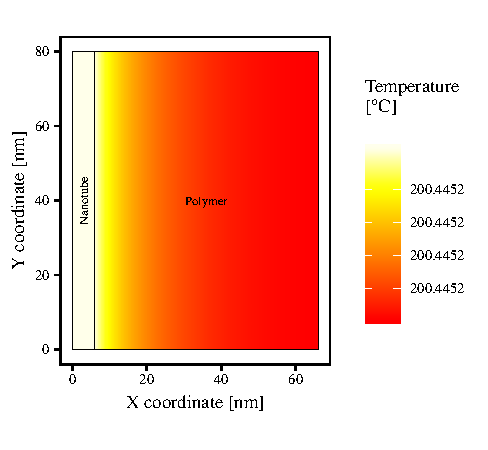
\includegraphics[width=0.45\textwidth]{resultats_comsol_axisymetrique_temp.pdf}
	} \qquad
	\subfigure[]
	{\label{fig:results_axysymmetric_b}
		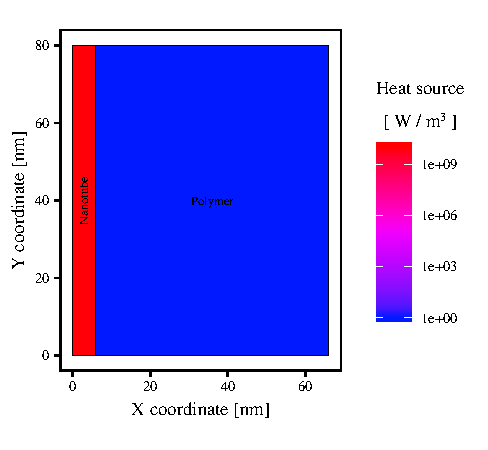
\includegraphics[width=0.45\textwidth]{resultats_comsol_axisymetrique_puissance.pdf}
	}
	\caption{Results of the FEM evaluating the heat generation within the MWCNT. The uniform temperature field is due to the short time constant for thermal diffusion in the model (see section \ref{sec:timeconstant}). a) uniform temperature field, b) heat generation field \cite{Brassard2018_figshare_article1}}
	\label{fig:results_axysymmetric}
\end{figure}

For the second FEM, the primary heat source was located at the contact point between the MWCNTs (Fig. \ref{fig:results_3D}b). 
Contribution from Joule heating within the MWCNTs was also present in the model with a power density 4 orders of magnitude lower. 
A uniform temperature profile is seen in MWCNTs, which is due to their high thermal conductivity. 
A uniform temperature of \SI{181}{\celsius} is obtained for this simulation after \SI{5}{\second} under an electric field of \SI{100}{\volt\per\metre}. 

\begin{figure}[h!]
	\centering
	\subfigure[]
	{\label{fig:results_3D_a} 								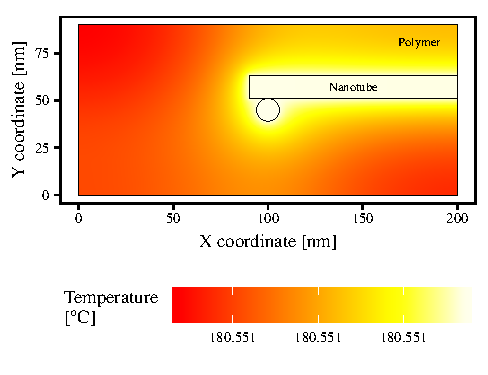
\includegraphics[width=0.45\textwidth]{resultats_comsol_3D_temp.pdf}
	} \qquad
	\subfigure[]
	{\label{fig:results_3D_b}
		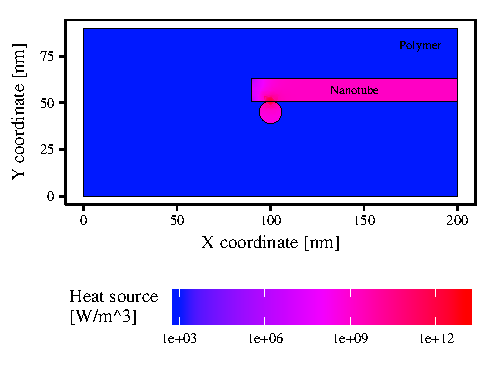
\includegraphics[width=0.45\textwidth]{resultats_comsol_3D_puissance_log.pdf}
	}
	\caption{Results of the FEM evaluating the effect of charge concentration and contact resistance. The uniform temperature field is due to the short time constant for thermal diffusion in the model (see section \ref{sec:timeconstant}) \cite{Brassard2018_figshare_article1}}
	\label{fig:results_3D}
\end{figure}
\FloatBarrier

In the third FEM, heat generation occurred almost exclusively in the polymer matrix (Fig. \ref{fig:result_gap}a and \ref{fig:result_gap}b). 
Heat is generated in the bulk of the polymer and a uniform temperature profile is obtained in the model (Fig. \ref{fig:result_gap}c and \ref{fig:result_gap}d). 

The third model demonstrates that the electric field required to reach a temperature similar to that of the first two models increases sharply when a small gap is introduced in the conductive network (Fig. \ref{fig:result_gap}). 
A gap of \SI{0.1}{\nano\metre}, between adjacent MWCNTs, required a field of \SI{9e9}{\volt\per\metre} to produce a temperature of \SI{185}{\celsius} (Fig. \ref{fig:result_gap}c). 
When the gap was increased to \SI{8}{\nano\metre} a field of \SI{5e10}{\volt\per\metre} was necessary to reach a similar temperature (Fig. \ref{fig:result_gap}d). 
These electrical field intensities are superior to the dielectric strength of PEI (\SI{3.3e7}{\volt\per\metre}) and the current went through the bulk of the polymer matrix. 
That seven order of magnitude increase in the electrical field, when a gap is introduced, confirms that the third heating mode is unlikely in practical applications. 
A connected network of MWCNTs provides pathways of lower resistance for the electrons to flow. 
A sharp increase in the resistance is indicative of a perturbation in the percolated network. 




\begin{figure}[h!]
	\centering
	\subfigure[]
		{\label{fig:result_gap_a} 								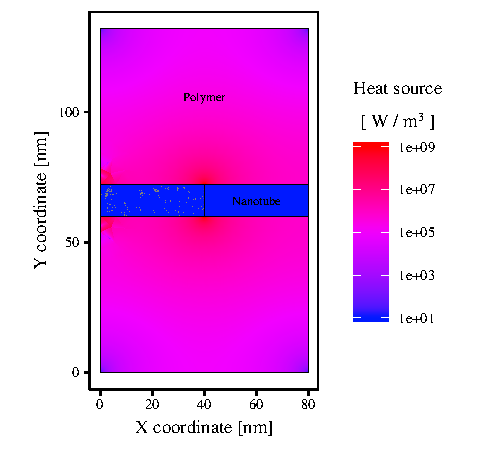
\includegraphics[width=0.46\textwidth]{resultats_0,1nm_comsol_2D_puissance.pdf}
		} 
	\subfigure[]
		{\label{fig:result_gap_b}
		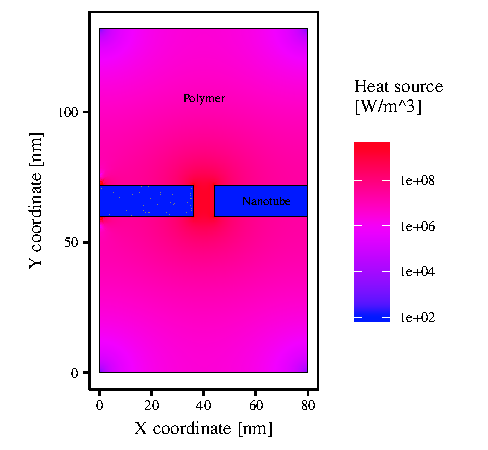
\includegraphics[width=0.46\textwidth]{resultats_8nm_comsol_2D_puissance.pdf}
		} \\
	\subfigure[]
		{\label{fig:result_gap_c} 								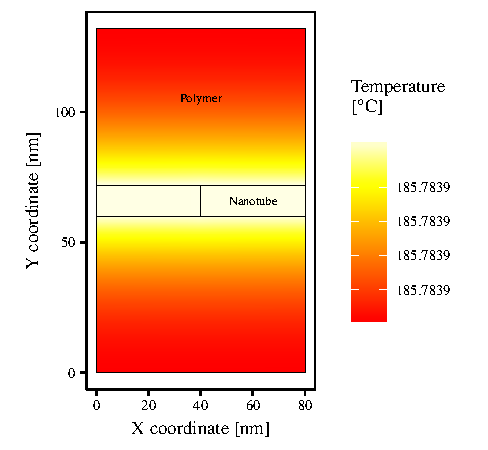
\includegraphics[width=0.46\textwidth]{resultats_0,1nm_comsol_2D_temp.pdf}
		} 
	\subfigure[]
		{\label{fig:result_gap_d}
		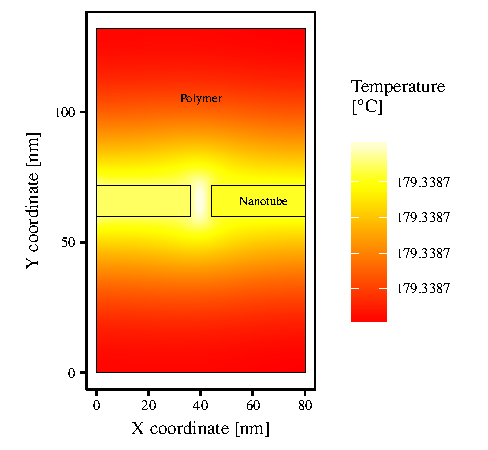
\includegraphics[width=0.46\textwidth]{resultats_8nm_comsol_2D_temp.pdf}
		}
	\caption{Effect of the gap length on the heat generation (a,b) and temperature fields (c,d) in the case of heat generation within the polymer. The uniform temperature fields are due to the short time constant for thermal diffusion in the model (see section \ref{sec:timeconstant}).  a) \SI{0.1}{\nano\metre} gap, \SI{9e9}{\volt\per\metre}, b) \SI{8}{\nano\metre} gap, \SI{5e10}{\volt\per\metre}, c) \SI{0.1}{\nano\metre} gap, \SI{9e9}{\volt\per\metre}, d) \SI{8}{\nano\metre} gap, \SI{5e10}{\volt\per\metre} \cite{Brassard2018_figshare_article1}}
	\label{fig:result_gap}
\end{figure}

From these results, we observe that conduction (and thus heat dissipation) within MWCNTs and through their contact points is the main driver for heat generation within a nanocomposite heating element. 
The uniform temperature fields observed at the constituent level lead to the conclusion that under normal operating conditions, local thermal degradation should not occur within the nanocomposite during the welding process. 

%%%%%%%%%%%%%%%%%%%%%%%%%%%%%%%%%%%%%%%%%%%%%%%%%%%%%%%%%%%%%%
\FloatBarrier
\subsection{Timescale analysis}
%%%%%%%%%%%%%%%%%%%%%%%%%%%%%%%%%%%%%%%%%%%%%%%%%%%%%%%%%%%%%%
\label{sec:timeconstant}

A comparative numerical analysis of the timescales for thermal diffusion, providing an explanation for the uniform temperature fields observed in the models, is presented in this section. 
Although PEI has poor thermal conductivity, uniform temperature fields with temperature variations not exceeding \SI{1e-5}{\celsius} are observed in the models. 
A comparative numerical analysis of the timescales for thermal diffusion, can explain this behaviour. 
This timescale is evaluated using the time constant for thermal diffusion ($t_D$) : 

\begin{equation}
t_D = \frac{L^2}{\alpha}
\label{equa:time_constant}
\end{equation}

\begin{figure}[htb]
	\center
	\captionsetup{width=35mm}
	%\resizebox{35mm}{!}{%\\
	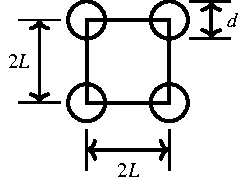
\includegraphics[scale=1]{arrangement_carre}
	%\tikzsetnextfilename{arrangement_carre}
	%\input{Tikz/arrangement_carre.tex}
	%}
	\caption{Square packing micromechanic model \cite{Brassard2018_figshare_article1}}
	\label{fig:square_packing}
\end{figure}

Assuming a uniform square packing of evenly distributed particles (Fig. \ref{fig:square_packing}) of known diameter ($d$) and variable volume fractions ($v_f$), it is possible to evaluate the average half distance ($L$) between particles :

\begin{equation}
L = \sqrt{\frac{\pi \ d^2}{16 \ v_f}}
\label{equa:L_average}
\end{equation}

The thermal diffusivity ($\alpha$) is defined as a function of thermal conductivity ($k$), density ($\rho$) and specific heat ($C_p$) : 

\begin{equation}
\alpha = \frac{k}{\rho \ C_p}
\label{equa:thermal_diffusivity}
\end{equation}

\begin{table}[htb]
	\centering
	\caption{Timescale for heat conduction}
	\begin{tabular}{@{}p{2.8cm}p{3.0cm}p{2.2cm}p{3.2cm}@{}}
		\toprule
		Weight fraction of MWCNTs & Volume fraction of MWCNTs & Average half distance & \textbf{Time constant}     \\
		$w_f$                     & $v_f$                     & L                     & $\mathbf{t_D}$             \\
		{[}\%{]}                  & {[}\%{]	}                 & {[}nm{]}              & \textbf{{[}s{]}}           \\ \midrule
		1                         & 0.65                      & 65.8                  & $\mathbf{3\times 10^{-8}}$ \\
		5                         & 3.31                      & 29.2                  & $\mathbf{6\times 10^{-9}}$ \\
		10                        & 6.74                      & 20.5                  & $\mathbf{3\times 10^{-9}}$ \\
		16                        & 11.02                     & 16.0                  & $\mathbf{2\times 10^{-9}}$ \\ \bottomrule
	\end{tabular}
	\label{tab:results_timescale}
\end{table}

Since the thermal conductivity of MWCNTs is very high compared to the polymer, only the properties of the matrix were considered in this timescale analysis. 
Table \ref{tab:results_timescale} presents the time constants calculated for thermal diffusion within the polymer matrix. 
The time constants varied from $3 \times 10^{-8}$ to \SI{2e-9}{\second} for $v_f$ varying from 1\% to 16\%. 
Considering that the simulations looked at Joule heating on a scale closer to the second, the short timescales for thermal diffusion explain the constant temperature fields. 

%%%%%%%%%%%%%%%%%%%%%%%%%%%%%%%%%%%%%%%%%%%%%%%%%%%%%%%%%%%%%%
\subsection{FTIR results}
%%%%%%%%%%%%%%%%%%%%%%%%%%%%%%%%%%%%%%%%%%%%%%%%%%%%%%%%%%%%%%

We collected FTIR spectra from a virgin PEI pellet, a nanocomposite PEI/MWCNT pellet, a nanocomposite film and two spectra from a fracture surface of a welded zone. 
The resulting absorbances spectra were calculated. 
The appearance of characteristic peaks, their position and width remained the same between the different spectra. 

\begin{figure}[h!]
	\center
	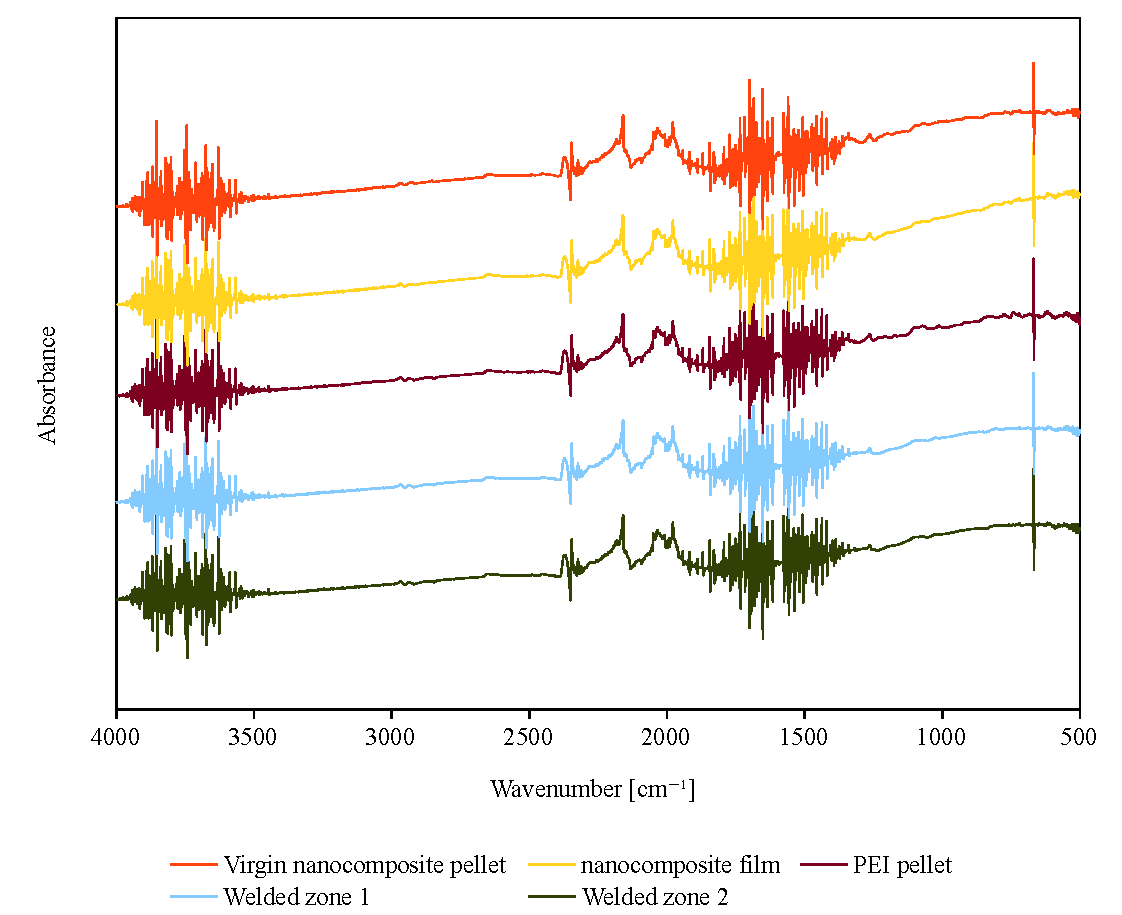
\includegraphics[width=0.8\textwidth]{FTIR_spectra.pdf}
	\caption{Raw FTIR spectra \cite{Brassard2018_figshare_article1}}
	\label{fig:FTIR_spectra}
\end{figure}
